\documentclass{article}
\usepackage[utf8]{inputenc}
\usepackage[T1]{fontenc}
\usepackage{amsmath}
\usepackage{xcolor}
\usepackage{amssymb}
\usepackage{pgfplots}
\usepackage{pgfplotstable}
\pgfplotsset{compat=1.7}
\usepackage{tikz}
\usetikzlibrary{positioning}
\usetikzlibrary{arrows}
\usepgfplotslibrary{fillbetween}

\begin{document}

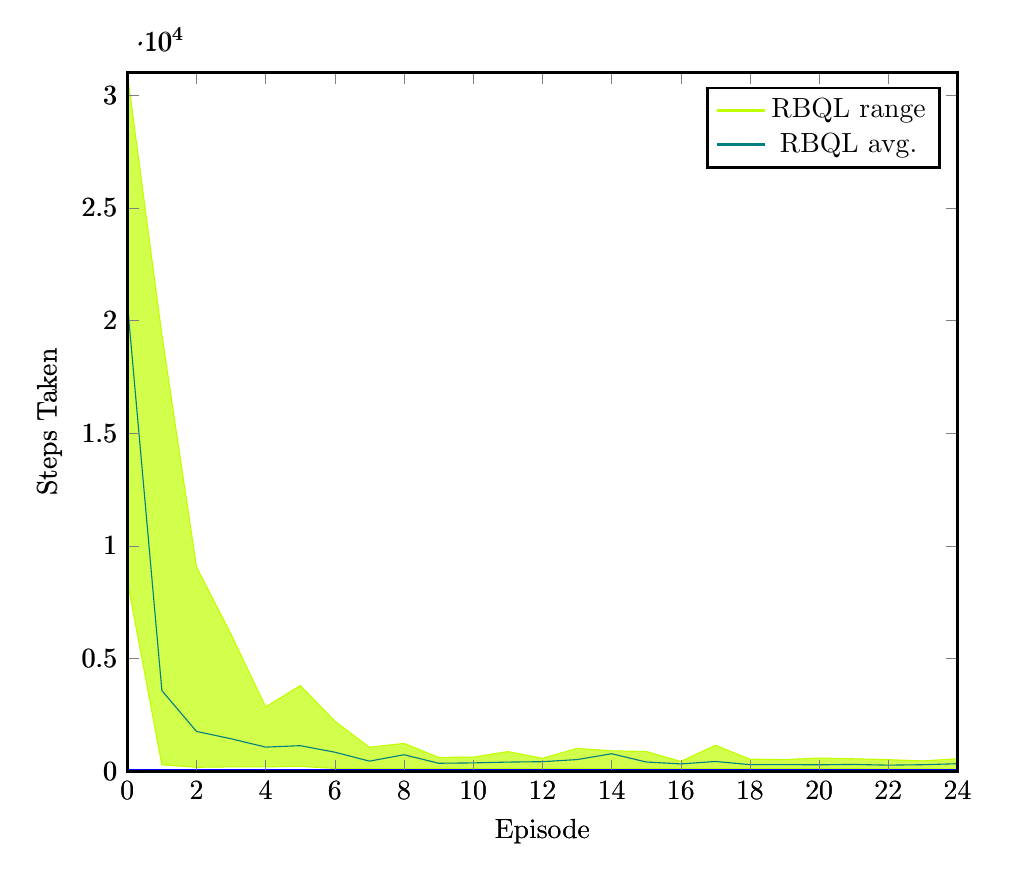
\begin{tikzpicture}
    \begin{axis}[ 
        width=\linewidth,
        line width=1,
        tick label style={font=\normalsize},
        legend style={nodes={scale=1, transform shape}},
        xlabel={Episode},
        ylabel={Steps Taken},
        ymin=0,ymax=31000,
        xmin=0,xmax=24
    ]

    \addplot[lime] coordinates{(0,0)};
    \addlegendentry{RBQL range};
    \addplot[teal] coordinates{(0,0)};
    \addlegendentry{RBQL avg.};

    \addplot[lime, name path=h] coordinates {
    (0,30947)(1,19358)(2,9072)(3,6081)(4,2864)(5,3810)(6,2232)(7,1075)(8,1246)(9,626)(10,635)(11,882)(12,584)(13,1023)(14,916)(15,884)(16,446)(17,1160)(18,546)(19,525)(20,596)(21,563)(22,524)(23,468)(24,565)
    };
    \addplot[lime, name path=i] coordinates {
    (0,8478)(1,295)(2,187)(3,205)(4,204)(5,228)(6,134)(7,130)(8,128)(9,140)(10,120)(11,126)(12,130)(13,134)(14,122)(15,122)(16,130)(17,122)(18,122)(19,122)(20,122)(21,122)(22,114)(23,116)(24,118)
    };
    \addplot[lime, opacity=0.7] fill between[of=h and i];

    \addplot[blue] coordinates {(0,98)(24,98)};

    \addplot[teal] coordinates {(0,20811.08)(1,3586.98)(2,1777.44)(3,1451.74)(4,1081.0)(5,1145.2)(6,855.68)(7,458.62)(8,742.4)(9,365.42)(10,381.38)(11,416.74)(12,435.14)(13,528.28)(14,787.32)(15,420.3)(16,336.34)(17,444.04)(18,303.8)(19,306.08)(20,296.3)(21,313.06)(22,281.12)(23,300.7)(24,344.9)};

    \end{axis}
    \begin{axis}[ 
        width=\linewidth,
        line width=1,
        tick label style={font=\normalsize},
        legend style={nodes={scale=1, transform shape}},
        xlabel={Episode},
        ylabel={Steps Taken},
        ymin=0,ymax=31000,
        xmin=0,xmax=24
    ]
    \end{axis}
\end{tikzpicture}

\end{document}